%------------------------------------------------------------------------------
% Template file for the submission of papers to IUCr journals in LaTeX2e
% using the iucr document class
% Copyright 1999-2013 International Union of Crystallography
% Version 1.6 (28 March 2013)
%------------------------------------------------------------------------------


% \documentclass[preprint]{iucr}
\documentclass{iucr}

\usepackage{siunitx}
\usepackage{color}
% \usepackage{amsmath,amssymb}
% \usepackage{amsfonts} 
\usepackage{mathtools}
\usepackage[normalem]{ulem}
% rotation table labels...
% see https://tex.stackexchange.com/questions/98388/how-to-make-table-with-rotated-table-headers-in-latex
\usepackage{adjustbox}
\usepackage{array}
\usepackage{booktabs}
\usepackage{multirow}

\usepackage{amsmath}
\usepackage{url}
\usepackage{tikz}
\usetikzlibrary{arrows.meta,calc}

% \usepackage{enumitem}
% \usepackage[normalem]{ulem}
% % srio..........
% \usepackage{multicol}
% \usepackage{graphicx}
\DeclareMathOperator{\sinc}{sinc}

\newcommand{\todo}[1]{{\color{red}[TODO: "#1'']}}
\newcommand{\remove}[1]{ {\color{blue} \sout{#1}}}
\newcommand{\inblue}[1]{{\color{blue}#1}}
\newcommand{\inred}[1]{{\color{red}#1}}
\newcommand{\ingreen}[1]{{\color{green}#1}}
\newcommand{\soutred}[1]{{\color{red}\sout{#1}}}
\newcommand{\lambdabar}{{\mkern0.75mu\mathchar '26\mkern -8.2mu\lambda}}

\definecolor{JSR_blue}{RGB}{51, 102, 154}
\newcommand{\jsrblue}[1]{\textcolor{JSR_blue}{#1}}

\newcolumntype{R}[2]{%
    >{\adjustbox{angle=#1,lap=\width-(#2)}\bgroup}%
    l%
    <{\egroup}%
}
\newcommand*\rot{\multicolumn{1}{R{90}{1em}}
}
%in preprint use 
% \newcommand{\whencolumns}[2]{#1}
% otherwise
% \newcommand{\whencolumns}[2]{#2}

\makeatletter
\@ifclasswith{iucr}{preprint}{
\newcommand{\whencolumns}[2]{#1}
}{
\newcommand{\whencolumns}[2]{#2}
}
\makeatother


 %-------------------------------------------------------------------------
 % Information about journal to which submitted
 %-------------------------------------------------------------------------
 \journalcode{X}              % Indicate the journal to which submitted
                              %   A - Acta Crystallographica Section A
                              %   B - Acta Crystallographica Section B
                              %   C - Acta Crystallographica Section C
                              %   D - Acta Crystallographica Section D
                              %   E - Acta Crystallographica Section E
                              %   F - Acta Crystallographica Section F
                              %   J - Journal of Applied Crystallography
                              %   M - IUCrJ
                              %   S - Journal of Synchrotron Radiation



\begin{document}                  % DO NOT DELETE THIS LINE

% \if@twocolumn
% \newcommand{\whencolumns}[2]{
% #2
% }
% \else
% \newcommand{\whencolumns}[2]{
% #1
% }
% \fi
% \makeatother

\title{Ray tracing mosaic crystals with SHADOW4}

\cauthor[1]{\jsrblue{Simone}}{\jsrblue{Manti}}{Simone.Manti@lnf.infn.it}{address if different from \aff}
\author[b]{\jsrblue{Manuel}}{\jsrblue{Sanchez del Rio}}
% \author[]{\jsrblue{Juan}}{\jsrblue{Reyes-Herrera}}

\aff[a]{INFN-LNF Frascati, \country{Italy}}
\aff[b]{ESRF - The European Synchrotron, 71 Avenue des Martyrs, 38000 Grenoble, \country{France}}

\maketitle                        % DO NOT DELETE THIS LINE

% -----------------------------------------------------------------
% -----------------------------------------------------------------

\begin{synopsis}
The model for mosaic crystals implemented in the ray tracing code SHADOW4 is
described. It combines a Monte Carlo sampling of the crystallite orientations,
which reproduces the focusing and defocusing properties of mosaic crystals, with
a reflectivity computed from the theory of mosaic crystals including secondary
extinction and beam penetration.
\end{synopsis}

% -----------------------------------------------------------------
% -----------------------------------------------------------------

\begin{abstract}
Mosaic crystals provide a wider reflectivity curve and a higher integrated
reflectivity than perfect crystals, making them suitable for optical systems
where luminosity, rather than energy resolution, is the limiting factor.
%This is the case for instruments that collect a large numerical aperture, such as crystal analyzers for X-ray emission spectroscopy, or monochromators for laboratory X-ray tubes and plasma sources.
We describe the model for mosaic crystals implemented in the ray tracing code SHADOW4 \cite{shadow4}. It is based on the model available in SHADOW since 1992, which is here revised, corrected and extended.
% The model is split into two independent steps: (i) a geometrical step that selects, for each ray, the orientation of the diffracting crystallite by Monte Carlo sampling of the mosaic distribution restricted to those orientations that satisfy Bragg's law, and (ii) a physical-optics step that computes the reflectivity from the theory of mosaic crystals, including secondary extinction. The penetration of the beam inside the crystal is sampled from a mean free path distribution, which is essential to reproduce the aberrations of thick mosaic crystals.
We discuss the improvements with respect to
the original implementation and the corrections introduced.
In particular, the orientation of the diffracting crystallite is now drawn from the
exact probability density of the azimuthal angle, including the Jacobian of the
change of variable, which removes, in principle, the assumption of a Gaussian
mosaic distribution, although only the Gaussian case is presently coded. The
validity limits of the model are also discussed. The code is also available in the graphical interface OASYS2-SHADOW4. We illustrate its use with some benchmarking and example cases.
\end{abstract}

% -----------------------------------------------------------------
% -----------------------------------------------------------------
\section{Introduction}
\label{sec:introduction}
% -----------------------------------------------------------------
% -----------------------------------------------------------------

Ray tracing simulations serve as essential tools for designing, optimizing, and
analyzing optical systems, providing invaluable insights into how light rays
propagate through intricate arrangements of optical components. Our interest lies
in revisiting and implementing mosaic crystals into the ray tracing SHADOW4
framework.

Mosaic crystals, such as graphite (HOPG, HAPG) or beryllium, are of interest
whenever a large integrated reflectivity is needed and a moderate energy
resolution is acceptable: pre-monochromators, monochromators for laboratory and
plasma sources, and, most notably, the large-solid-angle crystal analyzers used in
X-ray emission and inelastic scattering spectroscopy. Predicting the performance of
such systems requires a ray tracing code able to describe not only the wide
reflectivity curve, but also the very peculiar imaging properties of the mosaic
crystal: focusing in the diffraction plane, defocusing in the perpendicular plane,
and the aberrations introduced by the finite penetration of the beam.

A mosaic crystal is described in the model of \cite{zachariasen1945theory} as an
aggregate of a large number of small perfect crystallites, of microscopic or
submicroscopic size, oriented almost, but not exactly, parallel to each other. The
orientation of the lattice planes remains constant within a given crystallite, but
changes discontinuously when moving from one crystallite to another. The relative
displacements of the crystallites are assumed to be large compared with the
coherence width of the radiation, so that no defined phase relationship exists
between the waves scattered by the various crystallites. While the diffraction from
each crystallite is coherent, and must be treated with a full dynamical theory, the
scattering from the ensemble is incoherent with respect to it. In other words, the
mosaic crystal is an aggregate of independently scattering ideal crystals, and the
overall scattering can be described by a convolution process. The scattering planes
are defined by the direction of their normal, and the distribution of the normals of
the different crystallites is, to a good approximation, Gaussian with a standard
deviation $\kappa$ (the \emph{mosaicity} or \emph{mosaic spread}), ranging from about
$0.1^\circ$ to $0.5^\circ$ for graphite.

SHADOW, in its old version SHADOW2, already included a model for mosaic crystals
\cite{mosaicsSanchezDelRio1992, Scordo2021}. That code was inherited by SHADOW3
\cite{codeSHADOW} with only slight fixes, and a number of problems were identified
and corrected in an internal note \cite{mosaicsSanchezDelRio2013}. The present work
revises those algorithms and reimplements them in SHADOW4,
the new, fully object-oriented and python-based version of SHADOW, distributed
within the OASYS \cite{codeOASYS} environment.

Over the years the SHADOW mosaic model has been used in several research projects
(e.g. \cite{SanchezdelRio1998focusing}). Moreover, several groups have developed
other codes to perform ray tracing and Monte Carlo calculations with mosaic
crystals: the neutron package \emph{McStas} and its X-ray counterpart
\emph{McXtrace} \cite{Alianelli2004, BergbackKnudsen2013}, the Monte Carlo code
developed in Jena for von H\'amos spectrometers \cite{Zastrau2012, Zastrau2013},
the multiple-reflection model of Schlesiger and co-workers \cite{Schlesiger2017},
\emph{mmpxrt} \cite{Smid2021}, \emph{XICSRT} \cite{Pablant2021, Pablant2024} and,
most recently, \emph{HEART} \cite{Gawne2026}. Mosaic optics are also modelled in
the design and calibration of von H\'amos analyzers based on HOPG and HAPG
\cite{Scordo2021, Sokoltsova2022}. These codes are mostly
based on the original Darwin-Hamilton picture, whose exact solution for a mosaic
slab of finite thickness, in both the Bragg and the Laue geometry and for lattice
planes making an arbitrary angle with the surface, is known
\cite{Sears1997a, Sears1997b}. In these works additional effects
have been included, in particular multiple scattering inside the mosaic block
\cite{Wuttke2014, Bornemann2020, Schlesiger2017}, the
distinction between the mosaic-block angular distribution and the crystallite size
distribution, or intrinsic rocking-curve width
\cite{Gerlach2015, Smid2021, Alianelli2004}, and the description of highly
annealed pyrolytic graphite (HAPG) as a
stack of thin mosaic layers \cite{Zastrau2012, Zastrau2013}.

This recent literature suggests several directions in which the SHADOW model can be
extended, and it is useful to state from the outset which of them are addressed
here. The first, and for our purposes the most important, concerns the shape of the
mosaic distribution. Calibrated measurements on HAPG show that it is better
described by a Lorentzian, or even by a double Lorentzian, than by a Gaussian
\cite{Gerlach2015}, and Lorentzian mosaicities are adopted in several recent models
\cite{Schlesiger2017, Smid2021}; distributions defined on the unit sphere, such as
the von Mises-Fisher or a wrapped Lorentzian, have also been proposed
\cite{Gawne2026}. The reformulation of the geometrical step presented in
section~\ref{sec:geometry} makes no assumption on the shape of the mosaic
distribution, so that non-Gaussian and, in perspective, user-supplied or measured
distributions can be used (section~\ref{sec:geometry:nongaussian}). The conclusion
that the azimuthal angle, and not the angular deviation, is the correct variable to
sample has been reached independently in \cite{Gawne2026}.

A second direction is the treatment of multiple reflection inside the crystal,
described either as a small number of discrete internal reflections
\cite{Schlesiger2017}, as an explicit crystallite-by-crystallite random walk
\cite{Alianelli2004, Pablant2024, Gawne2026}, or through the generalized
Darwin-Hamilton transport equations \cite{Wuttke2014, Bornemann2020}. SHADOW4
retains here the macroscopic description, in which a single reflectivity accounts
for the ensemble of crystallites; its validity limits are discussed in
section~\ref{sec:penetration}. Curved mosaic crystals, required for the von H\'amos
and other focusing geometries, are already available in SHADOW4, because the mosaic
crystal is implemented as a crystal optical element and therefore inherits the
surface shapes of the code. The extension to the Laue (transmission) case and to
asymmetric cuts, for which the exact solution of the Darwin equations is known
\cite{Sears1997a}, and the possibility of adjusting the internal parameters of the
model, such as the reflecting power $Q$ or the secondary extinction, to fit
experimental data \cite{Alianelli2001}, are left for future work.

This paper aims to describe the revision of the algorithms and the new
implementation of mosaic crystals in SHADOW4. Section~\ref{sec:properties} recalls
the properties of mosaic crystals that a ray tracing code must reproduce.
Section~\ref{sec:geometry} describes the geometrical model that assigns a
diffraction direction to each ray, including the corrections to the original 1992
algorithm. Section~\ref{sec:reflectivity} describes the calculation of the
reflectivity, and section~\ref{sec:penetration} the treatment of the penetration
depth. The implementation in SHADOW4 is presented in
section~\ref{sec:implementation} and illustrated with examples in
section~\ref{sec:examples}.


% -----------------------------------------------------------------
\section{Properties and functions of mosaic crystals}
\label{sec:properties}
% -----------------------------------------------------------------

Two properties make the mosaic crystal qualitatively different from a perfect
crystal in a ray tracing simulation, and both are a direct consequence of the fact
that the diffracting planes are not unique but distributed. They are illustrated in
Fig.~\ref{fig:focusing}.

\begin{figure}
\centering
% Redrawn after Fig. 1 of Sanchez del Rio et al. (1998).
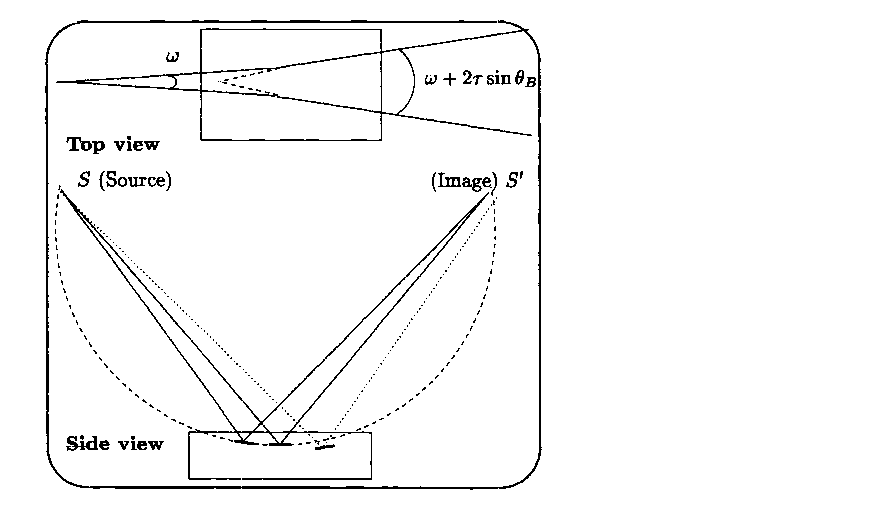
\includegraphics[width=0.95\columnwidth]{figures/mosaic_focusing_1998.pdf}
\caption{\emph{Top:} defocusing effect of a mosaic crystal in the plane
perpendicular to the diffraction plane. The incident divergence $\omega$ is
increased to $\omega + 2\tau\sin\theta_B$ due to the crystal mosaicity, $\tau$
being the mosaic spread expressed as FWHM. \emph{Bottom:} parafocusing
effect of a mosaic crystal in the diffraction plane. Several rays with the same
energy coming from the source point $S$ are diffracted by different crystallites
inside the mosaic crystal according to Bragg's law. This requires the ray to travel
inside the crystal until it finds a crystallite with the correct orientation. The
diffracted rays converge to a point $S'$ (assuming that the penetration depth and
the footprint on the crystal are much smaller than the source-crystal distance).
The crystal-$S'$ distance is equal to the $S$-crystal distance, thus the
parafocusing effect happens in a magnification ratio $1$:$1$. When another ray
(dotted) with the same energy encounters a crystallite deeper in the crystal, it is
reflected to a point close to but different from $S'$, producing a broadening of the
focal spot. The parafocusing effect can also be understood as produced by
crystallites that follow a curved surface (dashed circle), like a spherical mirror:
the crystallite orientation must follow the Rowland circle to assure that Bragg's
law is fulfilled, and therefore the $1$:$1$ magnification geometry is just a
consequence of the Rowland condition. Redrawn after
\cite{SanchezdelRio1998focusing}.}
\label{fig:focusing}
\end{figure}

\emph{(i) Focusing in the diffraction plane.} A monochromatic ray that hits a flat
mosaic crystal is diffracted only if it finds a crystallite whose normal satisfies
Bragg's law. Two rays that leave the same source point $S$ with the same energy but
different directions are therefore diffracted by \emph{different} crystallites, and
the diffracted rays converge to a single image point $S'$ when the source-crystal
and crystal-image distances are equal. A \emph{flat} mosaic crystal thus focuses
monochromatic radiation in the diffraction plane at the $1:1$ conjugate
(Fig.~\ref{fig:focusing}, bottom). In the same geometry a flat perfect crystal
simply reflects the beam, preserving the divergence.

\emph{(ii) Defocusing in the plane perpendicular to the diffraction plane.} The
crystallites lying in the perpendicular plane can have different orientations that
still satisfy Bragg's law, so that the divergence in that plane is increased by
$2\tau\sin\theta_B$ (Fig.~\ref{fig:focusing}, top). As a consequence the image is
not a point but a segment perpendicular to the diffraction plane, whose length grows
with the mosaicity and with the distance to the crystal.

A third, related, property is that the mosaic crystal behaves as a \emph{dispersive}
element: since the position of the focus in the diffraction plane depends on the
Bragg angle, a polychromatic point source is imaged into a set of spots, one per
energy, spatially separated at the focal plane. This opens the possibility of
increasing the energy resolution of a mosaic crystal monochromator by placing an
exit slit after it.

Finally, mosaic crystals are \emph{thick} optical elements. The penetration depth
can reach the millimetre range, so that the diffraction does not occur on a surface
but in a volume. This spoils the perfect focusing described in (i) and introduces
an aberration that has to be modelled (section~\ref{sec:penetration}).

A useful ray tracing model must therefore (a) assign to every ray a diffraction
direction sampled from the correct distribution of crystallite normals, (b) assign
a reflectivity, and (c) assign a depth at which the diffraction event takes place.
These three ingredients are described in the following sections.


% -----------------------------------------------------------------
\section{A model for the geometrical reflection of X-rays in a mosaic crystal}
\label{sec:geometry}
% -----------------------------------------------------------------

\subsection{Geometry and notation}
\label{sec:geometry:notation}

Consider an incident ray with unit wavevector direction $\mathbf{k}$ arriving at
the point $O$ of the crystal surface, whose (mean) normal is $\mathbf{n}$, pointing
along the $z$ axis (Fig.~\ref{fig:geometry}). We use the following angles, all of
them measured \emph{from the normals}:

\begin{figure}
\centering
% Redrawn after Fig. 2 of Sanchez del Rio et al. (1992).
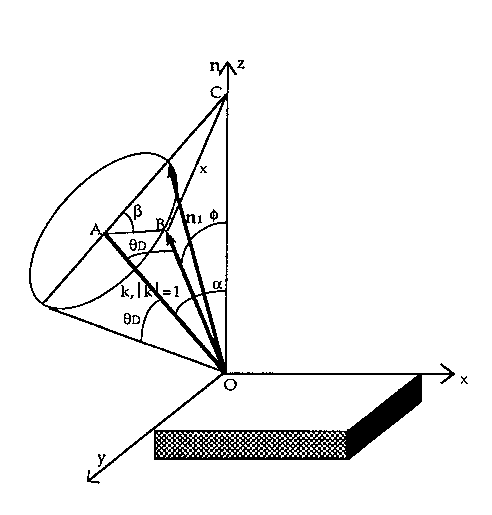
\includegraphics[width=0.8\columnwidth]{figures/mosaic_geometry_1992.pdf}
\caption{Ray tracing of an incident ray $\mathbf{k}$ on a mosaic crystal
(schematic). The crystal surface lies in the $xy$ plane and its mean normal
$\mathbf{n}$ is along $z$. The incident ray arrives at $O$ with an incidence angle
$\alpha$ measured from $\mathbf{n}$. The normals of all the crystallites that
satisfy Bragg's law lie on the cone of half-aperture $\theta_D$ around
$\mathbf{k}$; $\mathbf{n}_1$ is the most probable one (the one contained in the
diffraction plane) and the selected crystallite normal $\mathbf{OB}$ is obtained by
rotating $\mathbf{n}_1$ around $\mathbf{k}$ by the azimuthal angle $\beta$. The
angle between $\mathbf{OB}$ and $\mathbf{n}$ is $\phi$, the variable that follows
the mosaic distribution. The points $A$, $B$ and $C$ are the intersections with the
plane perpendicular to $\mathbf{k}$ at unit distance from $O$ of, respectively,
$\mathbf{k}$ itself, the selected crystallite normal $\mathbf{OB}$, and the surface
normal $\mathbf{n}$; hence $|AB| = \tan\theta_D$, $|AC| = \tan\alpha$, the angle
$BAC$ is $\beta$ and $x = |BC|$, which is the geometry underlying
equations~(\ref{eq:abc}) and (\ref{eq:boc}). Redrawn after
\cite{mosaicsSanchezDelRio1992}.}
\label{fig:geometry}
\end{figure}

\begin{itemize}
\item $\alpha$: the incidence angle, i.e. the angle between the incident ray and the
surface normal $\mathbf{n}$. It is the complement of the grazing angle.
\item $\theta_D$: the \emph{diffraction angle}, i.e. the angle between the incident
ray and the normal $\mathbf{OB}$ of the crystallite that satisfies Bragg's law. It
is the complement of the Bragg angle,
\begin{equation}
\lambda = 2 d \sin\theta_B = 2 d \cos\theta_D ,
\label{eq:bragg}
\end{equation}
and it is fixed by the photon energy and by the interplanar distance $d$ only.
\item $\phi$: the angle between the crystallite normal $\mathbf{OB}$ and the surface
normal $\mathbf{n}$; this is the variable that follows the mosaic distribution.
\item $\beta$: the azimuthal (dihedral) angle that orients $\mathbf{OB}$ on the cone
of half-aperture $\theta_D$ around $\mathbf{k}$.
\end{itemize}

The mosaic distribution of the crystallite normals around $\mathbf{n}$ is Gaussian,
\begin{equation}
w(\phi) = \left( \kappa \sqrt{2\pi} \right)^{-1} \exp\left( -\frac{\phi^2}{2\kappa^2} \right) ,
\label{eq:mosaic_distribution}
\end{equation}
where $\kappa$ is the mosaic spread (standard deviation); it is related to the
commonly quoted full width at half maximum by
$\kappa = \mathrm{FWHM}/(2\sqrt{2\ln 2})$.
%Some authors, and in particular the note \cite{mosaicsSanchezDelRio2013}, denote this quantity by $\tau$.

The normals of all those crystallites that would diffract the incident ray
according to Bragg's law can be visualized as a cone of half-aperture $\theta_D$
around $\mathbf{k}$. Among all these vectors we must select one, which must also
follow the random distribution law of
equation~(\ref{eq:mosaic_distribution}). Because $\mathbf{k}$, $\mathbf{n}$ and
$\mathbf{OB}$ form a spherical triangle, the four angles are not independent: the
spherical law of cosines gives
\begin{equation}
\cos\phi = \cos\alpha \, \cos\theta_D + \cos\beta \, \sin\alpha \, \sin\theta_D .
\label{eq:cosphi}
\end{equation}
Equation~(\ref{eq:cosphi}) is the central relation of the geometrical model. It is
a compact form, derived in \cite{mosaicsSanchezDelRio2013}, of the pair of
equations (2) and (3) of \cite{mosaicsSanchezDelRio1992}, which were obtained by
applying the plane cosine theorem to the triangles $ABC$ and $BOC$ of Fig.~\ref{fig:geometry},
\begin{eqnarray}
x^2 &=& \tan^2\theta_D + \tan^2\alpha - 2\tan\theta_D \tan\alpha \cos\beta , \label{eq:abc} \\
x^2 &=& \cos^{-2}\theta_D + \cos^{-2}\alpha - 2 \cos\phi/(\cos\theta_D \cos\alpha) , \label{eq:boc}
\end{eqnarray}
$x$ being the length of the segment $AC$.

Note that for $\beta = 0$ equation~(\ref{eq:cosphi}) reduces to
$\phi = |\alpha - \theta_D|$: the crystallite normal lies in the diffraction plane
and its tilt with respect to the surface is just the angular distance of the ray
from the nominal Bragg condition. It is therefore natural to define the rocking (or
deviation) angle
\begin{equation}
\Delta = \alpha - \theta_D ,
\label{eq:delta}
\end{equation}
which vanishes when the incident ray is at the exact Bragg angle for the mean
lattice orientation, and which is the argument of the reflectivity curve of
section~\ref{sec:reflectivity}.

Once $\mathbf{OB}$ is known the diffracted direction follows from the ordinary
reflection laws with respect to the crystallite: the angle of incidence equals the
angle of reflection, and incident ray, reflected ray and $\mathbf{OB}$ lie in the
same plane. This procedure is valid only if the distance on the crystal surface
between the interception points of different rays is larger than the crystallite
size, which is the usual case in a ray tracing calculation with a reasonable number
of rays.

%The same geometry can be formulated in reciprocal space instead of with the cone construction of Fig.~\ref{fig:geometry}, by requiring that the scattering vector match the reciprocal lattice vector of the crystallite,
%\begin{equation}
%\mathbf{k}_s - \mathbf{k} = \mathbf{B}_H = h\mathbf{b}_1 + k\mathbf{b}_2 + l\mathbf{b}_3 ,
%\label{eq:laue}
%\end{equation}
%with $hc/E = 2 d_H \sin\alpha_B$, and by tilting $\mathbf{B}_H$ according to the mosaic distribution. The two descriptions are equivalent; the formulation of equation~(\ref{eq:laue}) is the one adopted in some recent codes \todo{cite Gawne et al. (2026), HEART}, and it generalizes more naturally to crystals whose lattice is not aligned with the surface.

\subsection{Sampling the orientation of the diffracting crystallite}
\label{sec:geometry:sampling}

In \cite{mosaicsSanchezDelRio1992} the crystallite normal was obtained in two
steps: first, the most probable normal $\mathbf{n}_1$ was computed as the result of
rotating $\mathbf{n}$ by an angle $\alpha - \theta_D$ around an axis perpendicular
to both $\mathbf{k}$ and $\mathbf{n}$; then $\mathbf{n}_1$ was rotated around
$\mathbf{k}$ by an angle $\beta$ obtained from equations~(\ref{eq:abc}) and
(\ref{eq:boc}).
\todo{ REMOVE
after drawing $\phi$ from the Gaussian distribution $w(\phi)$ restricted, by the inversion method, to the interval $[\alpha - \theta_D, \alpha + \theta_D]$ of $\phi$ values accessible on the Bragg
cone. This procedure has two conceptual defects. First, the sampling variable is $\phi$, whereas the variable that parametrizes the set of admissible crystallites is $\beta$: drawing $\phi$ from its truncated distribution and then \emph{forcing} the ray to have that $\phi$ while satisfying Bragg's law does not reproduce the correct density in $\beta$, because the transformation $\beta \rightarrow \phi$ of
equation~(\ref{eq:cosphi}) is not linear and its Jacobian is ignored; the result is
a depletion of rays around the centre of the image, a ``hole'' that can already be
appreciated in Fig.~6 of \cite{mosaicsSanchezDelRio1992} and that is evident in
Fig.~1 of \cite{mosaicsSanchezDelRio2013}. Second, for a ray arriving far from the
nominal Bragg angle the inversion of equations~(\ref{eq:abc}) and (\ref{eq:boc})
becomes ill-conditioned and the algorithm fails to return an output direction.
A third problem, purely computational, was also present in SHADOW3: the code that
selects the sense (clockwise or counter-clockwise) of the rotation around
$\mathbf{k}$ did not update the random seed, so that the images produced were not
symmetric but lacked a part of the distribution; this was fixed in
\cite{mosaicsSanchezDelRio2013}. The two conceptual defects are cured by changing
the sampling variable, as described next.

Instead of drawing $\phi$ and solving for $\beta$, }

We first express the mosaic
distribution as a function of $\beta$ --- that is, we restrict it to the set of
crystallite normals that fit Bragg's law --- and then sample $\beta$ from it.
Substituting equation~(\ref{eq:cosphi}) into
equation~(\ref{eq:mosaic_distribution}),
\begin{eqnarray}
w\left( \phi(\beta) \right) &\propto& \exp\left( -\frac{[\phi(\beta)]^2}{2\kappa^2} \right) ,
\label{eq:wbeta} \\
\phi(\beta) &=& \arccos\left( \cos\alpha \cos\theta_D + \cos\beta \sin\alpha \sin\theta_D \right) .
\nonumber
\end{eqnarray}
This function of $\beta$ is not Gaussian, and its cumulative function is not
analytical. However, numerical calculations for several cases ranging from grazing
to normal incidence show that it is Gaussian to a very good approximation over the
range of $\beta$ that carries a significant probability. It is then convenient to
replace equation~(\ref{eq:wbeta}) by an approximating Gaussian, for which sampling
is trivial and already implemented in the code. Expanding $\phi^2$ in power series
around $\beta = 0$,
\begin{equation}
\phi^2(\beta) = s_0 + s_1 \beta^2 + o(\beta^4) ,
\label{eq:series}
\end{equation}
with
\begin{eqnarray}
s_0 &=& \arccos^2 C_0 ,
\label{eq:s0} \\
s_1 &=& \frac{\sin\theta_D \, \sin\alpha \, \arccos C_0}{\sqrt{1 - C_0^2}} ,
\label{eq:s1}
\end{eqnarray}
where
\begin{equation}
C_0 = \sin\theta_D \sin\alpha + \cos\theta_D \cos\alpha .
\label{eq:C0}
\end{equation}
The odd-order coefficients vanish, as required by the symmetry
$\beta \rightarrow -\beta$. The expansion (\ref{eq:series}) and the coefficients
(\ref{eq:s0}) and (\ref{eq:s1}) were obtained with a computer algebra
system\footnote{Starting from equations~(\ref{eq:abc}) and (\ref{eq:boc}), the
elimination of $x$ gives $\tan^2\theta_D + \tan^2\alpha - 2\tan\theta_D \tan\alpha
\cos\beta - \cos^{-2}\theta_D - \cos^{-2}\alpha + 2\cos\phi/(\cos\theta_D
\cos\alpha) = 0$, which simplifies to equation~(\ref{eq:cosphi}). The series
expansion of $\phi^2 = [\arccos(\cos\alpha\cos\theta_D +
\cos\beta\sin\alpha\sin\theta_D)]^2$ around $\beta = 0$ up to fourth order then
yields $s_0$ and $s_1$ of equations~(\ref{eq:s0}) and (\ref{eq:s1}), the
coefficients of $\beta$ and $\beta^3$ being zero.}.

Equation~(\ref{eq:C0}) is nothing but $C_0 = \cos(\alpha-\theta_D) = \cos\Delta$,
so that equations~(\ref{eq:s0}) and (\ref{eq:s1}) can be written in the more
transparent form
\begin{equation}
s_0 = \Delta^2 ,
\qquad
s_1 = \sin\theta_D \, \sin\alpha \, \frac{\Delta}{\sin\Delta} ,
\label{eq:s0s1_simple}
\end{equation}
which removes the apparent singularity: for $\Delta \rightarrow 0$ (a ray at the
exact Bragg angle for the mean lattice orientation)
$s_1 \rightarrow \sin\theta_D \sin\alpha$, and in addition, for a symmetric
reflection, $s_1 \rightarrow \sin^2\theta_D = \cos^2\theta_B$. This limit must be
coded explicitly to avoid a $0/0$ evaluation.

Introducing equation~(\ref{eq:series}) into equation~(\ref{eq:wbeta}), the $s_0$
term factors out as a multiplicative constant and the $s_1$ term gives the variance
of the approximating Gaussian:
\begin{equation}
p_\mathrm{G}(\beta) \propto \exp\left( -\frac{\beta^2}{2\kappa'^2} \right) ,
\qquad
\kappa' = \frac{\kappa}{\sqrt{s_1}} .
\label{eq:kappaprime}
\end{equation}
The azimuthal angle of the diffracting crystallite is therefore obtained with a
single draw from a normal distribution of zero mean and standard deviation
$\kappa'$, and the crystallite normal $\mathbf{OB}$ follows from rotating
$\mathbf{n}_1$ around $\mathbf{k}$ by that angle.
%The resulting images are symmetric and free from the central artifact (Figs.~2 and 3 of \cite{mosaicsSanchezDelRio2013}).

\todo{VERYFY or REMOVE It is worth stressing that the constant factor dropped in
equation~(\ref{eq:kappaprime}), $\exp(-s_0/2\kappa^2) = \exp(-\Delta^2/2\kappa^2)
\propto w(\Delta)$, is not lost: it is precisely the Gaussian weight that enters
the reflectivity through equation~(\ref{eq:eta}) below. The separation of the
model into a geometrical step (which fixes the \emph{direction} of the outgoing
ray) and a physical step (which fixes its \emph{intensity}) is thus consistent: the
probability that a ray at a deviation $\Delta$ from the Bragg angle finds a
suitable crystallite is accounted for once, in the reflectivity.}

\subsection{The exact probability density for Gaussian mosaicity}
\label{sec:geometry:exact}

Equation~(\ref{eq:kappaprime}) is an approximation in two distinct respects: the
power series~(\ref{eq:series}) is truncated at second order, and, more importantly,
the change of variable $\phi \rightarrow \beta$ has been applied to the
\emph{argument} of the distribution but not to its measure. The probability density
of $\beta$ that corresponds to a density $w(\phi)$ of the crystallite tilts is
given by the transformation rule
\begin{equation}
p(\beta) = w\left( \phi(\beta) \right) \left| \frac{\mathrm{d}\phi}{\mathrm{d}\beta} \right| ,
\label{eq:pbeta}
\end{equation}
and the Jacobian $|\mathrm{d}\phi/\mathrm{d}\beta|$ is missing from
equations~(\ref{eq:wbeta}) and (\ref{eq:kappaprime}). It can be obtained in closed
form. Introducing the shorthand
\begin{equation}
A = \cos\alpha \, \cos\theta_D , \qquad B = \sin\alpha \, \sin\theta_D ,
\label{eq:AB}
\end{equation}
equation~(\ref{eq:cosphi}) reads $\cos\phi = C(\beta) = A + B\cos\beta$, so that
$\phi(\beta) = \arccos C(\beta)$, defined for those $\beta$ that fulfil the
constraint $|A + B\cos\beta| \le 1$; the $C_0$ of equation~(\ref{eq:C0}) is
$C(0) = A + B$. From $\mathrm{d}C/\mathrm{d}\beta = -B\sin\beta$,
\begin{equation}
\left| \frac{\mathrm{d}\phi}{\mathrm{d}\beta} \right| =
   \frac{\sin\alpha \, \sin\theta_D \, |\sin\beta|}{\sqrt{1 - C^2(\beta)}} ,
\label{eq:jacobian}
\end{equation}
and, for the Gaussian mosaicity of equation~(\ref{eq:mosaic_distribution}), the
exact density of the azimuthal angle is
\begin{equation}
p(\beta) = \frac{1}{\kappa\sqrt{2\pi}}
   \exp\left( -\frac{\arccos^2 C(\beta)}{2\kappa^2} \right)
   \frac{\sin\alpha \, \sin\theta_D \, |\sin\beta|}{\sqrt{1 - C^2(\beta)}}
\label{eq:pbeta_exact}
\end{equation}
up to a normalization constant. \todo{Add the figure comparing
equation~(\ref{eq:pbeta_exact}) with the Gaussian approximation
of equation~(\ref{eq:kappaprime}) for HOPG~002 at 7058~eV with a mosaicity FWHM of
$0.1^\circ$, at the exact Bragg angle and at $\Delta = 3^\circ$ and $15^\circ$;
and the figure comparing the exact $\phi(\beta)$ with the two-term expansion
$\sqrt{s_0 + s_1\beta^2}$ and its residual (scripts in \texttt{develop/}).}

\subsection{Non-Gaussian mosaicity}
\label{sec:geometry:nongaussian}

Writing the density in the form~(\ref{eq:pbeta}) has a further advantage: it makes
no assumption on the shape of $w(\phi)$. Real mosaic crystals, and in particular
HOPG and HAPG, are not always well described by a Gaussian mosaicity; a Lorentzian
distribution of half width $\gamma$,
\begin{equation}
w(\phi) = \frac{1}{\pi} \frac{\gamma}{\phi^2 + \gamma^2} ,
\label{eq:lorentzian}
\end{equation}
or a Voigt distribution (the convolution of a Gaussian and a Lorentzian) often
represent the measured rocking curves better \cite{Gerlach2015, Smid2021}. For these, no closed-form Gaussian
surrogate such as equation~(\ref{eq:kappaprime}) is available and the sampling has
to be done by numerical inversion of the cumulative distribution,
\begin{equation}
F(\beta) = \frac{\displaystyle\int_{\beta_\mathrm{min}}^{\beta} p(\beta')\,\mathrm{d}\beta'}
                {\displaystyle\int_{\beta_\mathrm{min}}^{\beta_\mathrm{max}} p(\beta')\,\mathrm{d}\beta'} ,
\qquad
\beta = F^{-1}(u), \quad u \sim \mathcal{U}(0,1) ,
\label{eq:cdfinv}
\end{equation}
$[\beta_\mathrm{min}, \beta_\mathrm{max}]$ being the interval in which the
constraint $|A + B\cos\beta| \le 1$ is satisfied. This is the intended route for
SHADOW4: $F$ would be tabulated on a grid and inverted by interpolation, so that
Gaussian, Lorentzian and Voigt mosaicities could all be treated by the same code
path, equation~(\ref{eq:kappaprime}) being retained for the Gaussian case as a
fast analytical alternative. In the present implementation, however, only the
Gaussian case of equation~(\ref{eq:kappaprime}) is coded
(section~\ref{sec:implementation}). \todo{Update this paragraph, and add the
benchmark against the analytical Gaussian sampling, once the numerical inversion
is in place.}

\todo{Longer term: rather than assuming a functional form for $w(\phi)$, infer it
directly from measured rocking curves by Bayesian or maximum-likelihood fitting.}


% -----------------------------------------------------------------
\section{X-ray reflectivity of mosaic crystals}
\label{sec:reflectivity}
% -----------------------------------------------------------------

Once the direction of the diffracted ray is known, its intensity must be
multiplied by the crystal reflectivity. This is computed in the framework of the
theory of mosaic crystals (\cite{zachariasen1945theory,Bacon1948}), whose main idea
is to integrate the reflectivity curve of a single perfect crystallite over all the
possible orientations of the crystallites. In the Bragg (reflection) case, for a
crystal of thickness $t$, the diffracted intensity as a function of the rocking
angle $\Delta$ is\footnote {We use this equation in our development, which is restricted to the symmetric Bragg case (the crystal is in reflection geometry and the mean crystallite orientation coincides with the crystal normal). Asymmetric mosaic crystals are treated by \cite{Sears1997a}.}
\begin{equation}
r(\Delta) = \frac{a}{1 + a + \sqrt{1 + 2a} \, \coth\left( A\sqrt{1 + 2a} \right)} ,
\label{eq:reflectivity}
\end{equation}
with
\begin{equation}
a = \frac{w(\Delta) \, Q_{s,p}}{\mu} ,
\qquad
A = \frac{\mu t}{\sin\theta_B} ,
\label{eq:a_and_A}
\end{equation}
where $\mu$ is the linear absorption coefficient, $w(\Delta)$ is the mosaic
distribution of equation~(\ref{eq:mosaic_distribution}) evaluated at the deviation
angle of equation~(\ref{eq:delta}), and $Q_{s,p}$ is the reflecting power per unit
volume of the crystallite for the $s$ and $p$ polarization states. The quantity
$A$ is the absorption path in units of the absorption length.

The constants $Q$ for $s$ and $p$ polarization
are\footnote{Equations (6) and (7) of \cite{mosaicsSanchezDelRio1992} are
incorrect; they were corrected in \cite{mosaicsSanchezDelRio2013} and are given
here in the corrected form.}
\begin{eqnarray}
Q_s &=& \left( \frac{e^2}{mc^2} \frac{1}{v_0} \right)^2 \frac{|F_H|^2 \lambda^3}{\sin 2\theta_B} ,
\label{eq:Qs} \\
Q_p &=& Q_s \left( \cos 2\theta_B \right)^2 ,
\label{eq:Qp}
\end{eqnarray}
where $F_H$ is the structure factor of the reflection $H=(hkl)$, $v_0$ is the
volume of the unit cell, $\theta_B$ is the Bragg angle, $\lambda$ is the wavelength
of the radiation and $e^2/mc^2$ is the classical electron radius. In SHADOW4 it is
more convenient to write equation~(\ref{eq:Qs}) in terms of the Fourier components
of the electric susceptibility $\psi_H$ and $\psi_{\bar H}$, which are the
quantities returned by the crystal structure-factor libraries,
\begin{equation}
Q_s = \frac{\pi^2 \, | \psi_H \psi_{\bar H} |}{\lambda \, \sin 2\theta_B} ,
\label{eq:Qs_psi}
\end{equation}
an expression equivalent to equation~(\ref{eq:Qs}) that holds also for
non-centrosymmetric crystals. Similarly, the linear absorption coefficient is
obtained from the imaginary part of $\psi_0$ (\cite{zachariasen1945theory},
eq.~3.172),
\begin{equation}
\mu = -\frac{2\pi}{\lambda} \, \mathrm{Im}(\psi_0) .
\label{eq:mu}
\end{equation}

Equations~(\ref{eq:reflectivity})--(\ref{eq:mu}) hold under the following
approximations, which delimit the applicability of the model:
\begin{enumerate}
\item The top and bottom surfaces of the crystal are parallel, and also parallel to
the mean direction of the crystallites (symmetric Bragg geometry).
\item The mosaicity $\kappa$ is much larger than the rocking curve width of the
perfect crystallite (otherwise the convolution degenerates into the perfect crystal
case).
\item The radiation wavelength is much smaller than the crystallite size.
\item Primary extinction is negligible, which means that the crystallite size is
much smaller than the extinction length for primary extinction,
$t_\mathrm{ext} = v_0/(2 d F_H)$, $d$ being the distance between Bragg planes.
\end{enumerate}
\todo{Add the discussion of the more recent models that relax some of these
approximations (multiple scattering, layered HAPG, crystallite-size distribution),
and state which of them are implemented in SHADOW4.}

Figure~\ref{fig:diffraction_profiles} shows the diffraction profile of
equation~(\ref{eq:reflectivity}), computed with the quantities of
section~\ref{sec:implementation} for a HOPG~(002) crystal, $1$~mm thick, with a
mosaicity of $0.2^\circ$ FWHM, at $8$~keV. \emph{Top:} reflectivity as a function
of the deviation angle $\Delta$ at fixed energy. \emph{Bottom:} reflectivity as a
function of energy at the incidence angle fixed to the Bragg angle at $8$~keV,
obtained by converting $\Delta$ into an energy deviation through the local
dispersion $\mathrm{d}\theta_B/\mathrm{d}E$. Both panels are shown for the $s$
and $p$ polarization states, using the corresponding $Q_s$ and $Q_p$ of
equations~(\ref{eq:Qs_psi}) and (\ref{eq:Qp}). The angular width of the profile
($\sim 18'$ FWHM, broadened with respect to the $12'$ FWHM mosaic distribution by
the secondary-extinction factor $a$ of equation~(\ref{eq:a_and_A})) corresponds to
a much broader energy passband ($\sim 175$~eV FWHM) because of the shallow Bragg
angle ($13.4^\circ$) of this reflection.

\begin{figure}
\centering
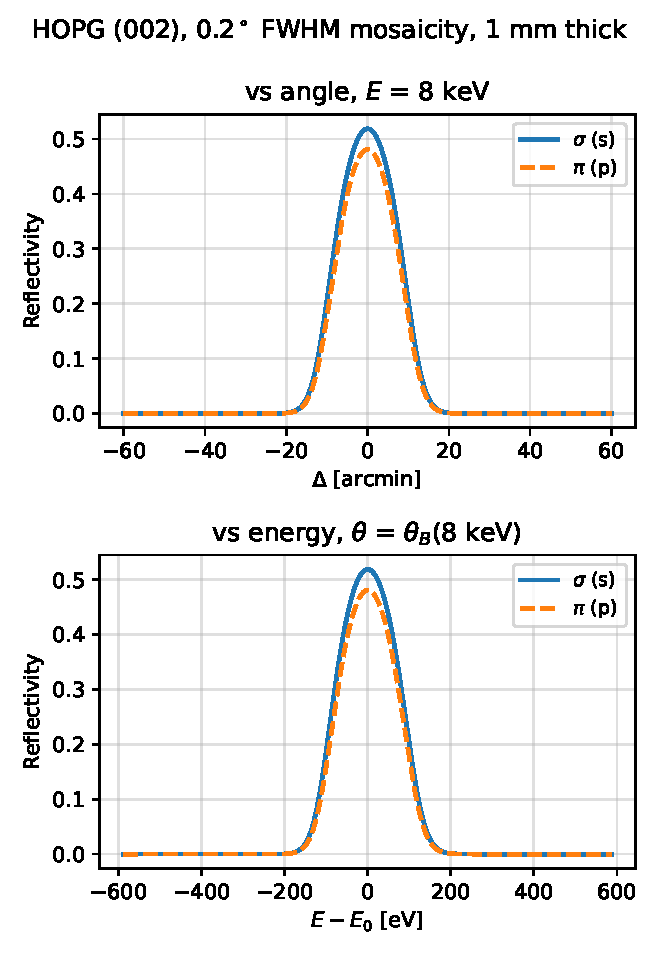
\includegraphics[width=0.8\columnwidth]{figures/diffraction_profiles_HOPG.pdf}
\caption{Diffraction profile of a mosaic HOPG~(002) crystal, $1$~mm thick, with a
Gaussian mosaicity of $0.2^\circ$ FWHM, computed from equation~(\ref{eq:reflectivity}).
\emph{Top:} reflectivity versus the deviation angle $\Delta$ at $8$~keV.
\emph{Bottom:} reflectivity versus energy, at the incidence angle fixed to the
Bragg angle at $8$~keV.}
\label{fig:diffraction_profiles}
\end{figure}


%In SHADOW3 the reflectivity curves were pre-computed by the utility \texttt{BRAGG}, which wrote a file containing all the mosaic parameters, and which supported the classical cubic cells and, additionally, the hexagonal close-packed and graphite cells. For a hexagonal cell described by the primitive vectors
%$\mathbf{a}_1 = a\mathbf{x}$, $\mathbf{a}_2 = (a/2)\mathbf{x} + (\sqrt{3}a/2)\mathbf{y}$ and $\mathbf{a}_3 = c\mathbf{z}$, the unit cell volume is $V = a^2 c \sqrt{3}/4$ and the distance between the planes defined by the Miller indices $(h,k,l)$ is
%\begin{equation}
%\frac{1}{d^2} = \frac{4}{3} \left[ \frac{h^2 + k^2 + hk}{a^2} \right] + \frac{l^2}{c^2} .
%\label{eq:dhex}
%\end{equation}
%The hexagonal close-packed structure has two atoms in the unit prism cell, locatedat $(0.33,0.67,0.25)$ and $(0.67,0.33,0.75)$; beryllium, for instance, has $a = 2.287$~\AA\ and $c = 3.583$~\AA. The graphite structure has four atoms in the unit prism, at $(0,0,0)$, $(0,0,0.5)$, $(0.33,0.67,0)$ and $(0.67,0.33,0.5)$, with $a = 2.456$~\AA\ and $c = 6.696$~\AA. In SHADOW4 this pre-processing step is no longer needed: the structure factors are computed on the fly (section~\ref{sec:implementation}).


% -----------------------------------------------------------------
\section{Secondary extinction: effect on penetration}
\label{sec:penetration}
% -----------------------------------------------------------------

A perfect focusing effect in the diffraction plane (property (i) of
section~\ref{sec:properties}) would be obtained only if the penetration depth
inside the crystal were negligible, or if each layer were to scatter coherently,
e.g. in phase. This is not the case in mosaic crystals, where penetration distances
as large as $1$~mm can be reached. A correct ray tracing program for mosaic
crystals must therefore include this penetration effect, which in turn requires
consideration of secondary extinction.

Following \cite{zachariasen1945theory}, secondary extinction is described by the
extinction coefficient (for $s$ and $p$ polarization)
\begin{equation}
\eta_{s,p} = w(\Delta) \, Q_{s,p} ,
\label{eq:eta}
\end{equation}
with $Q_{s,p}$ given by equations~(\ref{eq:Qs}) and (\ref{eq:Qp}) and $w$ by
equation~(\ref{eq:mosaic_distribution}). From this extinction coefficient one
obtains the penetration distance along the beam direction as the mean free path
\begin{equation}
\lambda_\mathrm{mfp} = \frac{1}{\eta_{s,p}} .
\label{eq:mfp}
\end{equation}
The penetration is then sampled ray by ray from $u \sim \mathcal{U}(0,1)$, which
gives the depth at which the diffraction event takes place. In the current
implementation the extinction coefficient entering the sampling is always
$\eta_s$, i.e. the mean free path is built on the $s$-polarization $Q_s$
regardless of the polarization state of the ray; extending the sampling to use
$\eta_p$ for $p$-polarized rays is left for future work. Because the ray cannot travel further
than the maximum path length $L = t/\sin\theta_B$ set by the crystal thickness
(the same $L$ that enters $A$ of equation~(\ref{eq:a_and_A})), the exponential
probability density of equation~(\ref{eq:mfp}) is truncated to the interval
$[0, L]$,
\begin{equation}
P(x) = \frac{\eta_{s,p}}{1 - \exp(-\eta_{s,p} L)} \exp(-\eta_{s,p} x) ,
\qquad 0 \le x \le L ,
\label{eq:penetration_pdf}
\end{equation}
and inverting its cumulative distribution gives
\begin{equation}
x = -\frac{1}{\eta_{s,p}} \ln\!\left[ 1 - u \left( 1 - e^{-\eta_{s,p} L} \right) \right] ,
\label{eq:penetration_sampling}
\end{equation}
which reduces to a uniform sampling on $[0, L]$ in the limit $\eta_{s,p} \to 0$.

The diffraction event is placed at the depth $x$ along the incident direction,
instead of at the crystal surface, and only then is the reflection geometry of
section~\ref{sec:geometry} applied and the outgoing ray propagated back to the
surface. As shown in Fig.~7 of \cite{mosaicsSanchezDelRio1992}, the resulting depth
distribution is an exponential decay whose characteristic length depends strongly
on the photon energy (a few tens of micrometres at 3~keV, a few hundred at 8~keV,
for graphite~002). It is this spread of diffraction depths that broadens the focal
spot of Fig.~\ref{fig:focusing} (bottom) and therefore limits the parafocusing.

Three points of the above procedure are worth making explicit. First, the mean
free path of equation~(\ref{eq:mfp}) is built on the extinction coefficient
$\eta_{s,p} = w(\Delta) Q_{s,p}$ of equation~(\ref{eq:eta}), following
\cite{mosaicsSanchezDelRio1992}, and not directly on $Q_{s,p}$: it is the
convolution of the reflecting power with the mosaic distribution, rather than the
reflecting power of a single crystallite, that sets the rate at which the beam is
depleted as it travels through the stack of crystallites. Second, the truncation
of equation~(\ref{eq:penetration_pdf}) to $[0,L]$ accounts for the finite crystal
thickness, but the absorption coefficient $\mu$ does not enter the sampling
density: $\mu$ already enters the reflectivity of equation~(\ref{eq:reflectivity})
through $A$ of equation~(\ref{eq:a_and_A}), which is evaluated over the full
thickness $t$ and not over the sampled depth $x$. Third, and as a consequence,
no additional attenuation along the exit path from $x$ back to the surface is
applied: the sampled depth $x$ only determines the geometrical aberration
described below, while the intensity of the ray is weighted by the
depth-integrated reflectivity of equation~(\ref{eq:reflectivity}), independently
of $x$. This decoupling of the geometrical and radiometric roles of the
penetration depth is a simplification with respect to the recent
multiple-scattering treatments \cite{Wuttke2014, Bornemann2020, Alianelli2004,
Pablant2024, Gawne2026}, in which absorption and secondary extinction compete
step by step along the photon path; reconciling the two descriptions is left for
future work.


% -----------------------------------------------------------------
\section{Implementation in SHADOW4}
\label{sec:implementation}
% -----------------------------------------------------------------

SHADOW4 is an object-oriented software package written in python. Every optical
element (mirror, crystal, lens) is represented by two associated classes: an
``optical element'', which holds the physical description of the component, and a
``beamline element'', which combines it with its coordinates in the beamline and
performs the ray tracing. Following this pattern, the mosaic crystal is
implemented by the class \texttt{S4MosaicCrystal} (an optical element), which
holds the crystal description --- material, Miller indices, thickness, asymmetry
angle, and the mosaicity FWHM and its distribution profile --- and by the class
\texttt{S4MosaicCrystalElement} (a beamline element), which performs the
diffraction of the beam.

In contrast with SHADOW3, where the crystal data had to be pre-computed and stored
in a file by the \texttt{BRAGG} pre-processor, SHADOW4 obtains the crystal
structure factors at run time through \texttt{crystalpy} and the \texttt{DABAX}
crystal and scattering-factor database. This removes the interpolation over a
pre-tabulated energy grid, and makes the hexagonal (graphite, beryllium) cells
available on the same footing as the cubic ones.

The interaction of the beam with the crystal, coded in the beamline-element
method \texttt{\_apply\_crystal\_diffraction}, follows the three steps described
above, implemented ray by ray in three independent methods:
\begin{itemize}
\item \texttt{\_calculate\_mosaic\_reflectivity} evaluates the closed-form,
finite-thickness reflectivity amplitude of equation~(\ref{eq:reflectivity}), for
the $s$ and $p$ polarizations, at the deviation angle $\Delta$ between the actual
incidence angle and the Bragg angle; it depends on the full crystal thickness $t$
through $A$ of equation~(\ref{eq:a_and_A}), and not on the sampled penetration
depth (section~\ref{sec:penetration});
\item \texttt{\_calculate\_mosaic\_reflection} samples the diffracted direction: it
first rotates the surface normal by $\Delta$ to obtain the most probable
crystallite normal $\mathbf{n}_1$, then samples the azimuthal angle $\beta$ from
the exact Gaussian density of equation~(\ref{eq:kappaprime}), with $s_1$ of
equation~(\ref{eq:s0s1_simple}) evaluated through its $\Delta \rightarrow 0$-safe
form, and rotates $\mathbf{n}_1$ around the incident direction by $\beta$;
\item \texttt{\_sample\_mosaic\_penetration} samples the truncated-exponential
penetration depth of equation~(\ref{eq:penetration_sampling}) and displaces the
ray accordingly.
\end{itemize}
A fourth method, \texttt{\_calculate\_jones\_and\_efield\_directions}, propagates
the Jones vector and the $s$- and $p$-polarization directions consistently with
the sampled outgoing direction and the two amplitude reflectivities above.
Following the same optical-element/surface-shape decorator pattern used for the
ordinary, non-mosaic SHADOW4 crystal classes, a full set of surface-shape
subclasses of \texttt{S4MosaicCrystal} is now available --- plane, sphere,
ellipsoid, toroid, paraboloid, hyperboloid, generic conic, and two
numerical-mesh variants (\texttt{S4PlaneMosaicCrystal}, \texttt{S4SphereMosaicCrystal},
\ldots\,) --- the same nine surface shapes offered for perfect crystals. Because
the three methods above query the optical surface generically, this parity
required no change to the diffraction physics, only the surface-shape decorator,
shared with the rest of SHADOW4; section~\ref{sec:VonHamos} illustrates a curved
(spherically bent cylindrical) mosaic crystal.

Three limitations of the current implementation should be stated explicitly.
First, only the symmetric Bragg cut is supported, consistently with the
restriction of section~\ref{sec:reflectivity}; an asymmetric cut raises a
\texttt{NotImplementedError}. Second, although the mosaic distribution profile is
already a constructor parameter of \texttt{S4MosaicCrystal} (Gaussian or
Lorentzian), only the Gaussian profile is presently coded into the reflectivity,
orientation-sampling and penetration-sampling methods; the numerical inversion of
equation~(\ref{eq:cdfinv}) needed for the Lorentzian and Voigt cases of
section~\ref{sec:geometry:nongaussian} is not yet available. Third, as discussed in
section~\ref{sec:penetration}, the penetration depth is sampled using only the
$s$-polarization extinction coefficient $\eta_s$. Unit tests for these classes, and
a systematic validation against SHADOW3 of the kind illustrated in
section~\ref{sec:examples}, are in progress.


% -----------------------------------------------------------------
\section{Benchmarks and examples}
\label{sec:examples}
% -----------------------------------------------------------------

\subsection{Plane mosaic crystals}
\label{sec:benchmark1}

As a first working example of the SHADOW4 implementation, we reproduce the
three-line-source dispersion example of \cite{mosaicsSanchezDelRio1992} (their
Fig.~6, see also Fig.~3 of \cite{mosaicsSanchezDelRio2013}), using the actual
\texttt{S4PlaneMosaicCrystal} / \texttt{S4PlaneMosaicCrystalElement} classes of
section~\ref{sec:implementation}. A point source, with a small and anisotropic
angular divergence ($\pm 0.5$~mrad in the plane perpendicular to the diffraction
plane, $\pm 0.1$~mrad in the diffraction plane) and three closely spaced energy
lines ($7996$, $8000$ and $8004$~eV), illuminates a plane HOPG~(002) mosaic
crystal, $1$~mm thick, with a Gaussian mosaicity of $0.2^\circ$ FWHM, set at the
Bragg angle for $8000$~eV. The source-crystal and crystal-image distances are
both $10$~m, i.e. the symmetric $1$:$1$ parafocusing geometry of Fig.~1 (bottom).
Figure~\ref{fig:dispersion} shows the resulting image, for $5000$ traced rays.

Of the $5000$ rays, none is geometrically lost, and the total intensity is
$2591$, i.e. an average reflectivity of $51.8\%$, in good agreement with the
$\sim 52\%$ peak reflectivity of the closed-form profile of
Fig.~\ref{fig:diffraction_profiles} computed independently in
section~\ref{sec:reflectivity} for the same crystal and energy --- a useful
cross-check between the per-ray Monte Carlo reflectivity of
section~\ref{sec:implementation} and the depth-integrated formula of
equation~(\ref{eq:reflectivity}). The image reproduces both properties of
section~\ref{sec:properties}: in the diffraction plane ($Z$), the three energy
lines are clearly resolved, $\sim 2.4$~mm apart (a dispersion of
$\sim 0.6$~mm/eV in this geometry) and individually only $\sim 0.26$~mm FWHM,
demonstrating the parafocusing of Fig.~\ref{fig:focusing} (bottom); in the
perpendicular plane ($X$), the three lines overlap into a single broad,
energy-independent blob of $\sim 21$~mm FWHM, the defocusing of
Fig.~\ref{fig:focusing} (top).

\begin{figure}
\centering
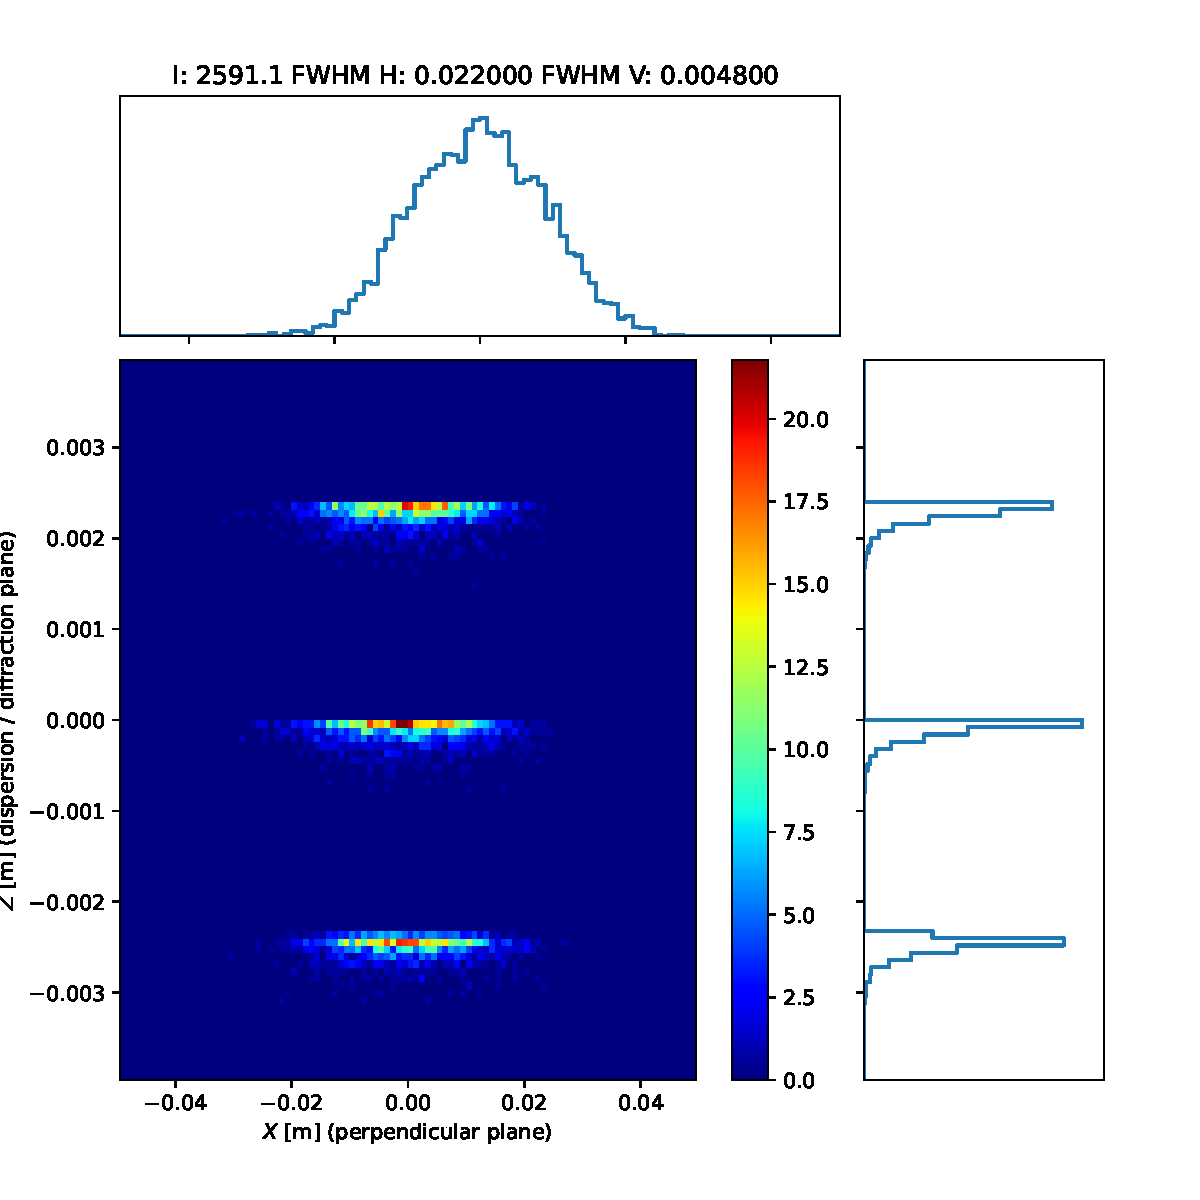
\includegraphics[width=\columnwidth]{figures/mosaic_crystal_flat_S4_dispersion.pdf}
\caption{Image at the focal plane of the three-line-source dispersion example of
section~\ref{sec:benchmark1}, ray-traced with SHADOW4 (\texttt{S4PlaneMosaicCrystal}):
a plane HOPG~(002) mosaic crystal, $1$~mm thick, $0.2^\circ$ FWHM Gaussian
mosaicity, in the symmetric $1$:$1$ geometry ($p=q=10$~m), for three energy lines
($7996$, $8000$, $8004$~eV) $4$~eV apart. The three lines are resolved in the
dispersion direction $Z$ and unresolved (defocused) in the perpendicular
direction $X$.}
\label{fig:dispersion}
\end{figure}

\todo{Complete this section with: (a) reflectivity curves of graphite~002 at 3, 8
and 17 keV for $0.4^\circ$ and $0.2^\circ$ FWHM mosaicity and 1 mm thickness
(their Fig.~3), compared with XOP \cite{SanchezdelRio2004}; (b) the change in
divergence of a monochromatic beam diffracted by a mosaic and by a perfect
crystal (their Fig.~4); (c) the cross section of the beam at the focusing plane
and downstream (their Fig.~5); (e) the penetration depth histograms (their
Fig.~7). Add a SHADOW3 vs SHADOW4 comparison and, if possible, a comparison
against experimental HOPG/HAPG data.}

\subsection{Rocking curves: effect of the source spectrum}
\label{sec:exampleRC}

A rocking curve is normally measured with a source of finite bandwidth, rather
than with a strictly monochromatic beam, and it is useful to know how much this
affects the observed curve. We use the crystal of section~\ref{sec:benchmark1},
rigidly tilted in steps around its nominal Bragg setting for $8000$~eV, and
retrace the same beamline of Fig.~\ref{fig:dispersion} at each tilt, for three
source photon-energy distributions: a monochromatic line, a box of $4$~eV width,
and a Lorentzian of $4$~eV FWHM --- the upper end of the $2$--$4$~eV range
typical of laboratory and plasma sources, chosen here to make the effect of the
bandwidth as visible as possible.

At the crystal's nominal mosaicity, $0.2^\circ$ FWHM, the monochromatic and
box-spectrum curves are indistinguishable: their peak intensities differ by
less than $0.01\%$ and their FWHM, $\sim 18'$, agrees with that of
Fig.~\ref{fig:diffraction_profiles}. The Lorentzian curve has the same FWHM
within the resolution of that scan, but a lower peak ($\sim 1.7\%$) and
integrated intensity ($\sim 0.3\%$), because its heavy tails place a small
fraction of the photons far enough from $8000$~eV that they do not satisfy
Bragg's law anywhere within the scanned range. This is because a $4$~eV
bandwidth corresponds, through the dispersion relation of
section~\ref{sec:benchmark1}, to an angular smearing of only $\sim 0.4'$, two
orders of magnitude smaller than this crystal's mosaic width: for this HOPG
crystal, a source bandwidth of a few eV has essentially no effect on the
observed rocking curve.

The effect should therefore become more visible as the crystal's own rocking
width is brought down towards this $\sim 0.4'$ smearing, but not brought down
too far: the model of section~\ref{sec:reflectivity} requires the mosaicity
to remain much larger than the rocking-curve width of the perfect crystallite
(the Darwin width, of order $50~\mu$rad $\approx 0.17'$ for a strong
reflection), and a mosaicity comparable to the Darwin width would leave the
mosaic-crystal approximation itself invalid. We therefore repeat the three-spectrum
comparison of Fig.~\ref{fig:rocking_curves} for a mosaicity of $0.05^\circ$
FWHM ($4$ times narrower than the nominal HOPG example, but still $\sim 17$
times the Darwin width), for which the monochromatic rocking curve has FWHM
$5.40'$. The three curves are now distinguishable, if only modestly so: the
box-spectrum curve remains indistinguishable from the monochromatic one (peak
and FWHM agree to better than $0.1\%$), while the Lorentzian curve has a
lower peak ($6706$ against $7155$, $-6.3\%$) and a slightly larger FWHM
($5.56'$, $+2.9\%$), with visibly heavier tails. This confirms, quantitatively,
that the source-spectrum effect on a measured rocking curve is controlled by
the ratio of the bandwidth-induced angular smearing to the crystal's own
rocking width, rather than by the bandwidth alone, but also that within the
range of mosaicities for which the model of section~\ref{sec:reflectivity}
applies, a few-eV source bandwidth remains a comparatively minor correction
for HOPG-like reflections.
\todo{Discuss cases in literature where the source bandwidth is comparable to,
or wider than, the crystal mosaicity. Think about how to fit experimental
data: which parameters to adjust (mosaicity? thickness? $Q_s$, as in Alianelli
2001, Fig.~3 and Table~3) once a measured rocking curve is available.}

\begin{figure}
\centering
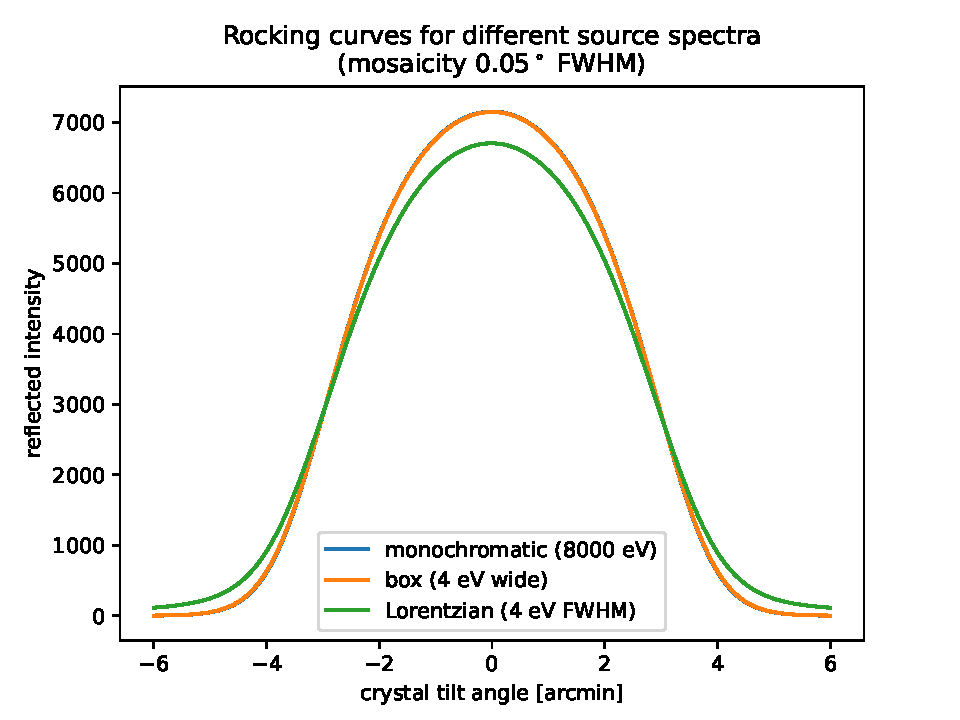
\includegraphics[width=0.9\columnwidth]{figures/rocking_curves_spectra.pdf}
\caption{Rocking curves of the plane HOPG~(002) mosaic crystal of
section~\ref{sec:benchmark1} ($1$~mm thick), with a Gaussian mosaicity reduced
to $0.05^\circ$ FWHM ($\sim 17$ times the Darwin width, still well within the
mosaic-crystal regime of section~\ref{sec:reflectivity}) to bring the
crystal's intrinsic rocking width closer to the scale of the
source-bandwidth-induced angular smearing, ray-traced with SHADOW4 for three
source photon-energy distributions centred at $8000$~eV: a monochromatic
line, a box of $4$~eV width, and a Lorentzian of $4$~eV FWHM. Unlike at the
crystal's nominal $0.2^\circ$ mosaicity (main text), the Lorentzian curve is
now visibly broader and lower than the monochromatic and box curves, which
remain indistinguishable from each other.}
\label{fig:rocking_curves}
\end{figure}

\subsection{Von H\'amos spectrometer}
\label{sec:VonHamos}

Unlike the Johann/Johansson spectrometer, which bends the crystal in the
diffraction (meridional) plane to focus point-to-point along the Rowland circle,
the von H\'amos spectrometer \cite{Szlachetko2012, Zastrau2012, Zastrau2013,
Sokoltsova2022} bends the crystal cylindrically in the plane
\emph{perpendicular} to the diffraction plane (the sagittal plane), leaving it
flat in the dispersion direction. A point source is then imaged, in the sagittal
plane only, onto a line on the detector, while different photon energies are
dispersed, undeflected by the meridional curvature, along the perpendicular
direction; a position-sensitive detector records the full spectrum in a single
exposure. Because the sagittal radius of curvature required for a given
source-to-crystal and crystal-to-detector distance is comparatively small (of
order metres rather than the tens of metres of a Rowland circle at the same
distances, equation~(\ref{eq:R_sagittal}) below), this geometry is well suited
to large-solid-angle collection with HOPG or HAPG mosaic crystals
\cite{Zastrau2012, Zastrau2013, Sokoltsova2022, Szlachetko2012}.

We simulate a sagittally-bent mosaic Si~(111) crystal at $8000$~eV
($\theta_B = 14.31^\circ$), with $p=q=10$~m. For a point-to-point sagittal focus,
the bending radius follows the standard grazing-incidence formula
\begin{equation}
R_\mathrm{sagittal} = \frac{2 \sin\theta_B}{1/p + 1/q} ,
\label{eq:R_sagittal}
\end{equation}
which for $p=q$ gives $R_\mathrm{sagittal} = p \sin\theta_B$. For our geometry
$R_\mathrm{sagittal} = 2.4714$~m.

Figure~\ref{fig:vonhamos}(a) shows the resulting image at the nominal $q=10$~m
plane for a mosaicity of $0.2^\circ$ FWHM: instead of the point-like sagittal
focus expected from equation~(\ref{eq:R_sagittal}), the image is an elongated,
essentially unfocused streak, $17$~mm FWHM in $X$.

\inred{REMOVE Two checks establish that
this is not a geometry or coding defect. First, the outgoing ray directions
computed by \texttt{\_calculate\_mosaic\_reflection} at the crystal surface
already encode the correct focusing kick: a linear fit of the sagittal
direction-cosine $v_X$ against the sagittal position $X$ on the crystal gives a
slope of $-0.0980$, matching the ideal point-focus value $-1/q = -0.1000$ to
within $2\%$. Second, repeating the simulation with the mosaicity as the only
free parameter, holding $p$, $q$ and $R_\mathrm{sagittal}$ fixed,
Fig.~\ref{fig:vonhamos}(b) shows that the image size scales linearly with the
mosaicity FWHM over more than two decades. The blur is therefore dominated by
the crystal's own mosaic spread, not by a geometrical aberration: with the
angular divergence of the source limited to $\pm 0.5$~mrad, the beam only
illuminates a narrow strip of the crystal, $\pm 5$~mm wide, around its centre
(a small fraction of the $\pm 100$~mm boundary allowed for this crystal); over
this strip, equation~(\ref{eq:R_sagittal}) only needs to bend the outgoing rays
by about $\pm 0.5$~mrad to focus them at $q$, an angular range comparable to,
or smaller than, the random deflection of order $1$--$2$~mrad that a
$0.2^\circ$ FWHM mosaic spread already imparts to individual rays through the
$\beta$ sampling of section~\ref{sec:geometry}. In other words, for a narrow,
weakly divergent source, the deterministic focusing signal is weak because it
only has a small range of crystal positions --- and hence a small range of
focusing angles --- to act on, and it is easily swamped by the crystal's
intrinsic angular spread; the image only becomes sharp once the mosaicity is
reduced well below the angular range subtended by the illuminated footprint at
$q$. }


This is consistent with the widely reported observation that the
resolution of real HOPG/HAPG-based von~H\'amos spectrometers is often limited
by the mosaic spread and the associated penetration-depth aberration rather
than by pure geometrical focusing \cite{Zastrau2012, Zastrau2013}, and it is a
useful, quantitative illustration of when a mosaic von~H\'amos design is, and
is not, aberration-limited.

The blur of Fig.~\ref{fig:vonhamos}(a,b) is a statement about the image at the
\emph{nominal} plane $q=10$~m; it leaves open whether the true focus (the
waist of the caustic) is still located there, only broadened, or whether it
has shifted elsewhere. 

\todo{ REMOVE We locate it by an analytic caustic scan: each ray is
forward- or back-projected from the image plane to a grid of propagation
distances $y$ around $q$, the intensity-weighted standard deviation of its
sagittal position $X(y)$ is computed at each $y$, and the $y$ of minimum
width is taken as the true focal position, refined to sub-grid accuracy by a
parabolic fit. }

Figure~\ref{fig:vonhamos}(c) shows the resulting shift $y-q$ as
a function of mosaicity, for the same crystals as panel (b): the true focus
moves \emph{closer to the crystal} as the mosaicity grows --- by as much as
$8.6$~m, for a beam meant to focus at $10$~m, when the mosaicity is
$0.2^\circ$ --- and the shift vanishes smoothly as the mosaicity tends to
zero, recovering the nominal $q$.

\todo{ REMOVE? This can be understood with the same
toy model as above: writing the sagittal ray coordinate at the crystal as
$x$ (variance $\sigma_x^2$, set by the illuminated footprint) and the
outgoing angle as $v_X = -x/q + n$, $n$ being the mosaic-induced random
deflection of variance $\sigma_n^2$, and propagating a distance $y$ from the
crystal, $X(y) = x(1-y/q) + yn$, so that
$\mathrm{Var}[X(y)] = (1-y/q)^2 \sigma_x^2 + y^2\sigma_n^2$ is minimized not
at $y=q$ but at $y^\ast = \sigma_x^2 q /(q^2 \sigma_n^2 + \sigma_x^2)$, which
tends to
$q$ as $\sigma_n \rightarrow 0$ and to a position closer to the crystal as
$\sigma_n$ grows relative to $\sigma_x/q$. Measuring $\sigma_x$ and $\sigma_n$
directly from the footprint of Fig.~\ref{fig:vonhamos}(a) (the standard
deviation of $X$ on the crystal, and the residual scatter of $v_X$ about the
linear fit of section~\ref{sec:VonHamos}, respectively) and inserting them in
$y^\ast$ reproduces the ray-traced shift to within a few percent, at every
mosaicity checked, and to $0.1\%$ at $0.2^\circ$.
The focal-position shift is
therefore not a separate
effect from the blur of panel (b), but the same mosaic-dominated regime seen
from the point of view of the caustic rather than of a fixed detector plane.
}

\begin{figure}
\centering
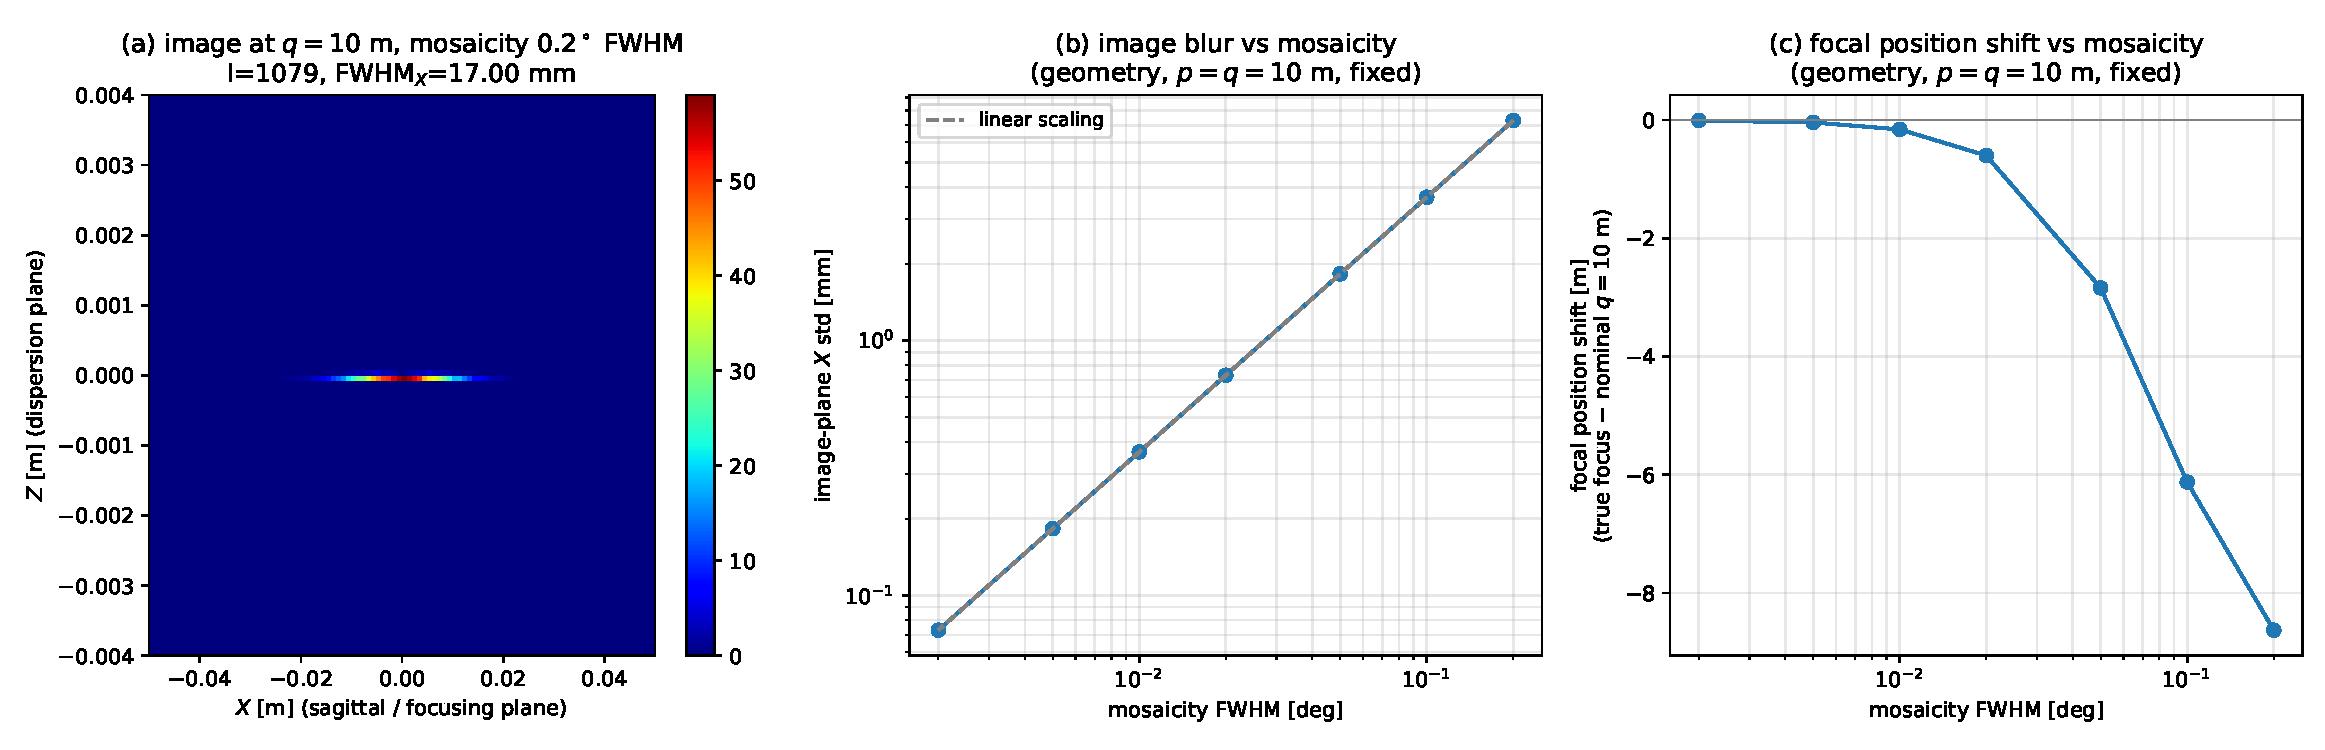
\includegraphics[width=\columnwidth]{figures/mosaic_crystal_vonhamos.pdf}
\caption{(a) Image at the nominal focal plane ($q=10$~m) of the sagittally-bent
mosaic Si~(111) von~H\'amos crystal of section~\ref{sec:VonHamos}, $0.2^\circ$
FWHM Gaussian mosaicity: the sagittal ($X$) direction is not sharply focused.
(b) Image-plane spread in $X$ as a function of the mosaicity FWHM, at fixed
geometry: the linear scaling shows that the blur in (a) is set by the mosaic
spread, not by a geometrical or coding defect. (c) Shift of the true focal
position (the caustic waist) with respect to the nominal $q=10$~m, as a
function of mosaicity: the focus moves closer to the crystal as the mosaicity
grows, and the shift vanishes as the mosaicity tends to zero.}
\label{fig:vonhamos}
\end{figure}

\todo{Search figures in literature that can be reproduced with our code (like Fig 5-7 in Gawne 2026) }




% -----------------------------------------------------------------
\section{Summary and conclusions}
\label{sec:summary}
% -----------------------------------------------------------------

We have revised the conceptual model for ray tracing calculations with mosaic
crystals originally proposed in \cite{mosaicsSanchezDelRio1992}, and reimplemented
it in SHADOW4. The model keeps the original two-step structure --- a geometrical
step that assigns the direction of the diffracted ray by Monte Carlo sampling of
the crystallite orientations, and a physical-optics step that assigns the
reflectivity from the theory of mosaic crystals of Zachariasen --- together with
the sampling of the penetration depth from the secondary extinction mean free path.

The main corrections with respect to the original implementation are: (i) the
sampling is now performed on the azimuthal angle $\beta$, using the probability
density obtained by restricting the mosaic distribution to the crystallite normals
that satisfy Bragg's law, which removes the non-physical holes in the ray
distribution and the failures for rays arriving far from the Bragg angle; (ii) that
density is now the exact one of equation~(\ref{eq:pbeta_exact}), which includes the
Jacobian of the transformation $\phi \rightarrow \beta$ omitted in
\cite{mosaicsSanchezDelRio2013}, the earlier Gaussian expression of
equation~(\ref{eq:kappaprime}) being kept as a fast analytical approximation;
(iii) the expressions for the reflecting powers $Q_s$ and $Q_p$ have been
corrected, and are now evaluated from the crystal susceptibilities computed at run
time; and (iv) the random number generation bug present in SHADOW3 is no longer
there.

Writing the sampling in terms of the exact density also removes, in principle, the
assumption of a Gaussian mosaicity: because equation~(\ref{eq:pbeta_exact}) makes
no assumption on the shape of $w(\phi)$, drawing the azimuthal angle by numerical
inversion of its cumulative distribution, equation~(\ref{eq:cdfinv}), would give
Lorentzian and Voigt mosaic distributions --- which often describe HOPG and HAPG
rocking curves better than a Gaussian \cite{Gerlach2015, Schlesiger2017, Smid2021}
--- at no extra conceptual cost. In the present implementation, however, only the
Gaussian case of equation~(\ref{eq:kappaprime}) is coded (section~\ref{sec:implementation});
completing the numerical inversion for the non-Gaussian case is the most direct
extension of this work, together with lifting the restriction to the symmetric
Bragg case and to the $s$-polarization extinction coefficient in the
penetration-depth sampling. The model is implemented as the
\texttt{S4MosaicCrystal} family of SHADOW4 optical-element and beamline-element
classes, which, sharing the surface-shape decorators of the ordinary crystal
classes, already supports curved mosaic crystals without any change to the
diffraction code.

The three examples of section~\ref{sec:examples} illustrate the implementation
and provide a first, informal validation. The three-line-source dispersion
example (section~\ref{sec:benchmark1}) reproduces the parafocusing and
defocusing properties of section~\ref{sec:properties}, and gives a ray-traced
average reflectivity ($51.8\%$) that agrees, at the percent level, with the
depth-integrated reflectivity computed independently from
equation~(\ref{eq:reflectivity}) for the same crystal and energy. The
rocking-curve comparison of section~\ref{sec:exampleRC} shows that, for this
HOPG crystal, a source bandwidth of a few eV --- typical of a monochromated
laboratory or plasma source --- has essentially no effect on the observed
rocking curve, only its far tails leaving a small trace; this quantifies when
the source spectrum, rather than the crystal itself, must be accounted for when
interpreting a measured rocking curve. The von~H\'amos example of
section~\ref{sec:VonHamos} shows that a mosaic-crystal spectrometer can be
geometrically correctly focused, in the sense that the sampled outgoing ray
directions already encode the ideal focusing condition, and yet appear
unfocused, because the mosaic spread dominates over a focusing signal that is
weak when the illuminated footprint is narrow; disentangling the two regimes,
as done there, is a prerequisite for a meaningful comparison with SHADOW3 or
with experimental data. Together with the extensions from the recent
literature discussed in section~\ref{sec:introduction} (non-Gaussian and
unit-sphere mosaic distributions, multiple reflection inside the crystal, and
the layered description of HAPG), a systematic, quantitative validation
against SHADOW3 and, where available, experimental HOPG/HAPG data remains the
main direction for future work. Longer term, inferring the mosaic distribution
directly from measured rocking curves, instead of postulating its functional
form (section~\ref{sec:geometry:nongaussian}), and completing the description
of the experiment by folding in the quantum efficiency curve of the detector,
would make the comparison with experimental spectra quantitative.


\newpage
\referencelist{iucr}

%-------------------------------------------------------------------------
% TABLES AND FIGURES SHOULD BE INSERTED AFTER THE MAIN BODY OF THE TEXT
%-------------------------------------------------------------------------

\end{document}                    % DO NOT DELETE THIS LINE
%%%%%%%%%%%%%%%%%%%%%%%%%%%%%%%%%%%%%%%%%%%%%%%%%%%%%%%%%%%%%%%%%%%%%%%%%%%%%%
